\documentclass[conference]{IEEEtran}
\IEEEoverridecommandlockouts
% The preceding line is only needed to identify funding in the first footnote. If that is unneeded, please comment it out.
\usepackage{cite}
\usepackage{amsmath,amssymb,amsfonts}
% \usepackage{algorithmic}
\usepackage{graphicx}
\usepackage{textcomp}
\usepackage{xcolor}

\usepackage{algorithm}
\usepackage{algpseudocode}

% \usepackage[usenames,dvipsnames]{color}
\usepackage{xcolor}

\usepackage{tabularx,booktabs}
\usepackage[flushleft]{threeparttable}

\def\BibTeX{{\rm B\kern-.05em{\sc i\kern-.025em b}\kern-.08em
    T\kern-.1667em\lower.7ex\hbox{E}\kern-.125emX}}
    
\usepackage{relsize}
\usepackage{scalerel}
\usepackage{tikz}
\usetikzlibrary{svg.path}

\definecolor{orcidlogocol}{HTML}{A6CE39}
\tikzset{
    orcidlogo/.pic={
        \fill[orcidlogocol] svg{M256,128c0,70.7-57.3,128-128,128C57.3,256,0,198.7,0,128C0,57.3,57.3,0,128,0C198.7,0,256,57.3,256,128z};
        \fill[white] svg{M86.3,186.2H70.9V79.1h15.4v48.4V186.2z}
        svg{M108.9,79.1h41.6c39.6,0,57,28.3,57,53.6c0,27.5-21.5,53.6-56.8,53.6h-41.8V79.1z M124.3,172.4h24.5c34.9,0,42.9-26.5,42.9-39.7c0-21.5-13.7-39.7-43.7-39.7h-23.7V172.4z}
        svg{M88.7,56.8c0,5.5-4.5,10.1-10.1,10.1c-5.6,0-10.1-4.6-10.1-10.1c0-5.6,4.5-10.1,10.1-10.1C84.2,46.7,88.7,51.3,88.7,56.8z};
    }
}

\newcommand\orcidicon[1]{\href{https://orcid.org/#1}{\mbox{\scalerel*{
                
\begin{tikzpicture}[yscale=-1,transform shape]
                \pic{orcidlogo};
                \end{tikzpicture}
            }{|}}}}

% \usepackage{hyperref} %<--- Load after everything else
\usepackage[colorlinks = true,
            linkcolor = blue,
            urlcolor  = magenta,
            citecolor = green,
            anchorcolor = blue]{hyperref} %<--- Load after everything else
    
\begin{document}

% \title{Conference Paper Title*\\
% {\footnotesize \textsuperscript{*}Note: Sub-titles are not captured in Xplore and
% should not be used}
% \thanks{Identify applicable funding agency here. If none, delete this.}
% }

\title{POCS-based Clustering Algorithm\\
% {\footnotesize \textsuperscript{*}Note: Sub-titles are not captured in Xplore and
% should not be used}
\thanks{*Corresponding Author}
}

% \title{POCS-based Clustering Algorithm
% }

\author{\IEEEauthorblockN{Le-Anh Tran$^{\textsuperscript{\orcidicon{0000-0002-9380-7166}}}$}
\IEEEauthorblockA{\textit{Dept. of Electronics Engineering} \\
\textit{Myongji University}\\
Gyeonggi, South Korea \\
leanhtran@mju.ac.kr}
\and
\IEEEauthorblockN{Henock M. Deberneh}
\IEEEauthorblockA{\textit{Dept. of Biochemistry and Molecular Biology} \\
\textit{University of Texas Medical Branch}\\
Texas, United States \\
henockmamo54@gmail.com}
\and
\IEEEauthorblockN{Truong-Dong Do$^{\textsuperscript{\orcidicon{0000-0001-8178-0018}}}$}
\IEEEauthorblockA{\textit{Dept. of Aerospace Engineering} \\
\textit{Sejong University}\\
Seoul, South Korea \\
dongdo@sju.ac.kr}
\and
\IEEEauthorblockN{Thanh-Dat Nguyen$^{\textsuperscript{\orcidicon{0000-0002-7098-5816}}}$}
\IEEEauthorblockA{\textit{Dept. of Research and Development} \\
\textit{OCST Co., Ltd.} \\
Seoul, South Korea \\
thanhdat6716@gmail.com}
\and
\IEEEauthorblockN{My-Ha Le}
\IEEEauthorblockA{\textit{Dept. of Electrical and Electronics Engineering} \\
\textit{HCMC University of Technology and Education}\\
Ho Chi Minh City, Vietnam \\
halm@hcmute.edu.vn }
\and
\IEEEauthorblockN{Dong-Chul Park*}
\IEEEauthorblockA{\textit{Dept. of Electronics Engineering} \\
\textit{Myongji University}\\
Gyeonggi, South Korea \\
parkd@mju.ac.kr}

% \IEEEauthorblockN{6\textsuperscript{th} Given Name Surname}
% \IEEEauthorblockA{\textit{dept. name of organization (of Aff.)} \\
% \textit{name of organization (of Aff.)}\\
% City, Country \\
% email address or ORCID}
}

\maketitle

\begin{abstract}
A novel clustering technique based on the projection onto convex set (POCS) method, called POCS-based clustering algorithm, is proposed in this paper. The proposed POCS-based clustering algorithm exploits a parallel projection method of POCS to find appropriate cluster prototypes in the feature space. The algorithm considers each data point as a convex set and projects the cluster prototypes parallelly to the member data points. The projections are convexly combined to minimize the objective function for data clustering purpose. The performance of the proposed POCS-based clustering algorithm is verified through experiments on various synthetic datasets. The experimental results show that the proposed POCS-based clustering algorithm is competitive and efficient in terms of clustering error and execution speed when compared with other conventional clustering methods including Fuzzy C-Means (FCM) and K-Means clustering algorithms. Code is available at: \url{https://github.com/tranleanh/pocs-based-clustering} 
\end{abstract}

\begin{IEEEkeywords}
POCS, clustering, unsupervised learning, machine learning, K-Means
\end{IEEEkeywords}


\section{Introduction}

Projection onto convex set (POCS) is a powerful tool for signal synthesis and image restoration which was originally introduced by Bregman in the mid-1960s \cite{b1}. The POCS method has been widely used to find a common point of convex sets in several signal processing problems. The main target of the POCS approach is to find a vector that resides in the intersection of convex sets. Bregman has shown that successive projections between two or more convex sets with non-empty intersection converge to a point that exists in the intersection of the convex sets. In the case of disjoint closed convex sets, the sequential projection does not converge to a single point, instead it converges to greedy limit cycles which are dependent on the order of the projections \cite{b1}. This property of POCS, however, can be applied to clustering problems. 

Clustering is an unsupervised data analysis technique that categories similar data points while separating them from the different ones \cite{b2}. Most clustering algorithms try to find homogeneous subgroups that have similar characteristics by the type of metric employed. The K-Means clustering algorithm, which has been one of the most popular methods for general clustering purposes \cite{b9}, uses the Euclidean distance to measure the similarity \cite{b2}. The K-Means clustering algorithm alternates between assigning cluster membership for each data point to the nearest cluster center and computing the center of each cluster as the prototype of its member data points. The objective of the K-Means clustering algorithm is to find a set of prototypes that minimize the cost function. The K-Means clustering algorithm terminates its training procedure when there is no further change in the assignment of instances to clusters \cite{b2}. The convergence of the K-Means clustering algorithm heavily depends on the initial prototypes. However, there exists no efficient and universal method for identifying the initial partitions \cite{b3}. Furthermore, the K-Means algorithm is known to be sensitive to noise and outliers \cite{b2}. In the Fuzzy C-Means (FCM) clustering algorithm \cite{b4}, on the other hand, a data point can belong to multiple subgroups simultaneously. The degree of certainty for a data point belonging to a certain cluster is represented by a membership function. The performance of the FCM algorithm is highly dependent on the selection of the initial prototypes and the initial membership value \cite{b4}. Furthermore, the drawbacks of the FCM clustering algorithm include extended computational time, incapability in handling noisy data and outliers \cite{b4}. In order to improve the convergence speed and the computation complexity of the FCM algorithm, the Gradient-Based Fuzzy C-Means (GBFCM) algorithm \cite{b5} was introduced by Park and Dagher which combines FCM and the characteristics of Kohonen’s Self Organizing Map \cite{b6} to improve performance.

In this paper, we propose a novel clustering algorithm using the convergence property of POCS. The proposed POCS-based clustering algorithm considers each data point as a convex set and projects the prototypes of the clusters to each of its constituent instances to compute a new set of center points. At first, the proposed algorithm initializes \textit{k} cluster prototypes. Based on the distance to the prototypes, each data point is assigned to one of the clusters which have the minimum distance from the data point. The cluster prototypes are projected to the member data points and combined convexly to minimize the objective function and the algorithm computes a new set of prototypes.


The remainder of this paper is structured as follows. Section II briefly reviews the POCS method. POCS-based clustering algorithm is proposed in Section III. In Section IV, the performance of the proposed POCS-based clustering algorithm on various synthetic datasets is examined and compared with those of other conventional clustering methods. Finally, Section V concludes the paper.


% \section{Related Works}

% \subsection{K-Means Clustering Algorithm}

% The IEEEtran class file is used to format your paper and style the text. All margins, 
% column widths, line spaces, and text fonts are prescribed; please do not 
% alter them. You may note peculiarities. For example, the head margin
% measures proportionately more than is customary. This measurement 
% and others are deliberate, using specifications that anticipate your paper 
% as one part of the entire proceedings, and not as an independent document. 
% Please do not revise any of the current designations.

% \subsection{Fuzzy C-Means Clustering (FCM) Algorithm}

% The IEEEtran class file is used to format your paper and style the text. All margins, 
% column widths, line spaces, and text fonts are prescribed; please do not 
% alter them. You may note peculiarities. For example, the head margin
% measures proportionately more than is customary. This measurement 
% and others are deliberate, using specifications that anticipate your paper 
% as one part of the entire proceedings, and not as an independent document. 
% Please do not revise any of the current designations.

% \subsection{Gradient-based FCM (GBFCM) Algorithm}

% The IEEEtran class file is used to format your paper and style the text. All margins, 
% column widths, line spaces, and text fonts are prescribed; please do not 
% alter them. You may note peculiarities. For example, the head margin
% measures proportionately more than is customary. This measurement 
% and others are deliberate, using specifications that anticipate your paper 
% as one part of the entire proceedings, and not as an independent document. 
% Please do not revise any of the current designations.

% \subsection{Density Peaks Clustering (DPC) Algorithm}

% The IEEEtran class file is used to format your paper and style the text. All margins, 
% column widths, line spaces, and text fonts are prescribed; please do not 
% alter them. You may note peculiarities. For example, the head margin
% measures proportionately more than is customary. This measurement 
% and others are deliberate, using specifications that anticipate your paper 
% as one part of the entire proceedings, and not as an independent document. 
% Please do not revise any of the current designations.


\section{The POCS Method}

\subsection{Convex Set}

\begin{figure}[t]
\centering
\includegraphics[width=0.7\columnwidth]{figures/fig1_v4.png}
\caption{Projection onto convex set: the projection of $x$ onto $A$ is the unique element in $A$ which is closest to $x$ and is denoted as $y$.}
\end{figure}

The theory of convex set has a rich history and has been a focus of research. It has been one of the most powerful tools in the theory of optimization \cite{b1}. A convex set is a collection of data points having the following property: given a non-empty set $A$ which is the subset of a Hilbert space $H$, $ A \subseteq H $ is called convex, for  $ \forall x_1, x_2 \in A $ and $\forall \lambda \in [0, 1]$, if the following holds true:

\begin{equation}
x := \lambda x_1 + (1 - \lambda)x_2 \in A  \label{eq1}
\end{equation}

Note that if $\lambda = 1$, $x = x_1$, and if $\lambda = 0$, $x = x_2$. For any value of $0 \leq \lambda \leq 1$ and $ x \in A $, $x$ lies on the line segment joining $x_1$ and $x_2$ when the set is convex.


\subsection{Projection onto Convex Set}
The concept of projection of a point to a plane deals with the optimization problem of interest, which is finding a point on the plane that has a minimum distance from the center of projection. For a given point $ x \notin A $, the projection of $x$ onto $A$ is the unique point $ y \in A $ such that the distance between $x$ and $y$ is a minimum. If $ x \in A $, then the projection of $x$ onto $A$ is $x$. The constrained optimization task can be expressed as:

% \eqref{eq2}
\begin{equation}
y = argmin || x - y^* ||^2  \label{eq2}
\end{equation} where $y^*$ is all the points on the set $A$. The projection onto a convex set is illustrated in Fig. 1.


\subsection{Alternating Projection onto Convex Sets}

\begin{figure}[t]
\centering
\includegraphics[width=1.0\columnwidth]{figures/fig2_v3.png}
\caption{Alternating POCS converges to a limit cycle for disjoint convex sets.}
\end{figure}

Alternating projection between two or more convex sets with non-empty intersection converges to a point that resides in the intersection of the convex sets. This prominent property of POCS can be applied to solve many optimization tasks, which can be described under the convex restriction sets. When $c_i$, $1 \leq i \leq n$, represents $n$ constraints with a non-empty intersection, the solution to the task resides in the intersection of the convex sets, which is expressed as: 

% \eqref{eq3}:

\begin{equation}
c_0 = \bigcap_{i=1}^{n}c_{i}  \label{eq3}
\end{equation}

Given the convex sets $c_i$, $ 1  \leq i \leq n$, which are closed and convex with a non-empty intersection, the successive projections on the sets will converge to a point that belongs to the intersection. Equation \eqref{eq4} denotes the algorithm, where $x_0$ is any point and represents the starting point, and $P_c$ is a projection operator onto $c$.

\begin{equation}
x_{k+1} = P_{c_n}...P_{c_2}P_{c_1}x_k \label{eq4}
\end{equation}

When these convex sets are disjoint, the sequential projection does not converge to a single point. Instead, it converges to greedy limit cycles which are dependent on the order of the projections. Fig. 2 depicts a geometrical visualization of the alternating POCS for three disjoint convex sets.


\subsection{Parallel Projection onto Convex Sets}

\begin{figure}[t]
\centering
\includegraphics[width=0.9\columnwidth]{figures/fig3_v3.png}
\caption{Graphical interpretation of parallel POCS for disjoint convex sets.}
\end{figure}

In the parallel mode of POCS, the initial point is projected to all convex sets simultaneously. Each projection has a weight and is combined convexly to solve the minimization problem. For a set of $n$ convex sets $C = \{ c_i | 1 \leq i \leq n \}$, the weighted simultaneous projections can be computed as follows:

\begin{equation}
x_{k+1} = x_k + \sum_{i=1}^{n} w_i (P_{c_i} - x_k) , k=0,1,2,... \label{eq5}
\end{equation} 

\begin{equation}
\sum_{i=1}^{n} w_i = 1 \label{eq6}
\end{equation} where $P_{c_i}$ is the projection of $x_k$ onto convex set $c_i$ and $w_i$ is the weight of importance of the projection. Note that $x_k$ represents the $k^{th}$ projection of the initial point $x_0$. The projection continues until convergence. The main advantages of the parallel mode of POCS when compared with the alternating one include computational efficiency and improved execution time.

If the sets are disjoint convex sets, the parallel form of POCS converges to a point that minimizes the weighted sum of the squares of distances to the sets. Suppose that the projection converges to a point $x^{*}$ such that the distance $d$ defined by \eqref{eq7} is minimized. A graphical illustration of the convergence of the parallel POCS method is presented in Fig. 3.


\begin{equation}
d = \sum_{i=1}^{n} w_i || x^{*} -  P_{c_i}(x^{*}) ||^2   \label{eq7}
\end{equation}


\section{POCS-based Clustering Algorithm}

% As mentioned in the previous section, the iterative projections (alternating or parallel) onto convex sets with non-empty intersection weakly converges to a point that resides on the intersection of the sets. For disjoint sets, the alternating POCS converges to a greedy limit cycle, the parallel mode of projection converges to a point that minimizes the weighted sum of the squared distance. In this study, we propose a clustering algorithm that utilizes the parallel form of POCS. The proposed POCS-based clustering algorithm considers each data point as a convex set and all data points in the cluster as disjoint convex sets. 

% The purpose of the algorithm is to find a point that minimizes the sum of the square of distances from each data point and the objective function $J$ for this purpose can be expressed as follows:

% \begin{equation}
% J = \sum_{j}^{k} \sum_{i=1}^{n} w_i || x_i -  P_{c_i}(x_i) ||^2   \label{eq8}
% \end{equation}

% \begin{equation}
% w_i = \frac{|| x_i - d_i ||}{\sum_{j=1}^{n}  || x_j - d_i || }   \label{eq9}
% \end{equation} with a constraint

% \begin{equation}
% \sum_{i=1}^{n} w_i = 1  \label{eq10}
% \end{equation} where $P_{c_k} (x_i)$ is the projection of the cluster center $x_i$ onto the member point $d_i$ and $w_i$ denotes the weight of importance of the projections while $x_i$ represents the $i^{th}$ member data point for the clusters.


% Following the definition of the convex set [12], empty set $\emptyset$, singleton set $ \{x_0\} $, line segments, hyperplanes, and Euclidian balls are considered as a convex set.

% A data point is a singleton set with only one element denoted by $ \{x_0\} $ and it is considered as a convex set. Let $V$ be a vector space over $R$, and let $x_0 \in V$. Then the singleton S = $ \{x_0\} $ is a convex set.

As mentioned in the previous section, the iterative projections (alternating or parallel) onto convex sets with non-empty intersection weakly converges to a point that resides on the intersection of the sets. For disjoint sets, the alternating POCS converges to a greedy limit cycle, the parallel mode of projection converges to a point that minimizes the weighted sum of the squared distances. In this study, we propose a clustering algorithm that utilizes the parallel form of POCS. The proposed POCS-based clustering algorithm considers each data point as a convex set and all data points in the cluster as disjoint convex sets. The objective function of the proposed POCS-based clustering algorithm is defined as:

% Consequently, we can devise the  POCS-based clustering algorithm to minimize the weighted sum of squared distances between the cluster prototypes and the member data points of the corresponding clusters. The objective function of the proposed POCS-based clustering algorithm is defined as:

\begin{equation}
J = argmin \sum_{j}^{k} \sum_{i=1}^{n} w_i || x_j -  P_{c_i}(x_j) ||^2   \label{eq11}
\end{equation}

\begin{equation}
w_i = \frac{|| x_j - d_i ||}{\sum_{p=1}^{n}  || x_j - d_{p} || }   \label{eq9}
\end{equation} with a constraint

\begin{equation}
\sum_{i=1}^{n} w_i = 1  \label{eq10}
\end{equation} where $k$, $n$ represents the number of clusters and the number of data points in one cluster, respectively, while $P_{c_i} (x_j)$ is the projection of the cluster prototype $x_j$ onto the member point $d_i$ and $w_i$ denotes the weight of importance of the projection.

At first, the algorithm initializes cluster prototypes as in K-Means++ \cite{b7} and assigns each data point to the nearest cluster center. Until convergence, the algorithm computes new cluster prototypes using \eqref{eq12} with a constraint as in \eqref{eq13}. The simultaneous  projections of the prototype $x_k$, where $k$ is the iteration index, continue until convergence. Starting from an initial point $x_0$, the projections converge to a point, $x_\infty$, that can minimize the weighted sum of the squares of distances.


\begin{algorithm}[t]
% \caption{POCS-based Clustering Algorithm}\label{alg:cap}
\caption{POCS-based Clustering Algorithm}
\begin{algorithmic}[1]
% \Require $n \geq 0$
% \Ensure $y = x^n$
\State Initialize cluster prototypes $x_{k,0} (k = 1, 2, ..., K)$,
\State Assign each data $d$ to its closest prototype,
\State $n \gets 1$,
\While{$n < N$}

    \For {$k = 1$ to $K$}
    \State $x_{k,n} \gets x_{k,n-1}$
        \For {$i = 1$ to $I_k$}
        
            \State $w_i \gets \mathlarger{\frac{|| x_{k,n-1} - d_i ||}{\sum_{j=1}^{I_k}  || x_{k,n-1} - d_j || }}$
            
            \State $x_{k,n} \gets x_{k,n} + w_i(d_i - x_{k,n-1})$
            
        \EndFor
    \EndFor

    \If {$x_{k,n} == x_{k,n-1}, \forall k$}
        \State break     \Comment{converged!}
    \EndIf

\EndWhile
\end{algorithmic}
\end{algorithm}


\begin{equation}
x_{k+1} = x_k + \sum_{i=1}^{n} w_i (P_{c_i} - x_k), k=0,1,2,... \label{eq12}
\end{equation}

\begin{equation}
\sum_{i=1}^{n} w_i = 1  \label{eq13}
\end{equation}

% The clustering problem we are dealing with is to solve the optimization problem for the objective function given by \eqref{eq11}. It implies that the clustering problem of our interest is to find clusters on given data points based only on L2-norm between any two vector points and there does not exist a class or predetermined cluster for a given data. This clustering problem can be considered as unsupervised learning and deals only with convex clustering problems.

\section{Experiments and Results}

% TABLE 1
\begin{table}[t]
\caption{Synthetic datasets.}
\setlength\tabcolsep{0pt} % make LaTeX figure out intercolumn spacing
\begin{tabular*}{\columnwidth}{@{\extracolsep{\fill}} lccc}

\toprule
     \textbf{Dataset} & \textbf{Number of Clusters} & \textbf{Attributes} & \textbf{Instances} \\

\midrule
     A1  & 20 & 2 & 3,000 \\
     A2  & 35 & 2 & 5,250 \\
     S1  & 15 & 2 & 5,000 \\
     S2  & 15 & 2 & 5,000 \\
     R15  & 15 & 2 & 600 \\
     Aggregation  & 7 & 2 & 788 \\
     
\bottomrule
\end{tabular*}
\end{table}

In order to evaluate the effectiveness of the proposed POCS-based clustering algorithm, various experiments on a variety of synthetic datasets have been conducted. The experiments exploits publicly available synthetic datasets that are available on the website “Clustering datasets” \cite{b8}. These experiments aim to thoroughly explain the convergence property of the proposed algorithm in terms of visual clustering results,
execution speed, and clustering error. The specifications of the datasets are summarized in Table I.

% \subsection{Results on Gaussian Datasets}

% The experiments on the Gaussian datasets were conducted by the following three phases. The first phase dealt with a clustering task of 1,000 data points that belong to two clusters. The dataset for the second experiment was comprised of four clusters with 250 data points each and the dataset for the last phase experiments consisted of six clusters with a total of 1,000 data points. The distributions of the datasets are depicted in Fig. 4. In order to evaluate the performance of the proposed POCS-based clustering algorithm in comparison with K-Means algorithm, convergence speed and execution time were adopted as performance measures. Fig. 5 shows the comparison in terms of clustering error and the number of training epochs. The clustering error was calculated as the sum of distances between the cluster center and member points. The Processor used in the experiments was Intel(R) Core\textsuperscript{TM} i7-4790K CPU @ 4.00GHz on a 64-bit operating system.

% \begin{figure}[t]
% \centering
% \includegraphics[width=1.0\columnwidth]{figures/gaussian_all_results.png}
% \caption{Results of POCS-based clustering algorithm on randomly generated Gaussian distribution datasets with (a) two clusters (b) four clusters (c) eight clusters.}
% \end{figure}

% \textcolor{red}{As can be seen from the results shown in Fig. 5, both P-POCS and A-POCS algorithms converge faster than the FCM algorithm in most of the cases. As the number of clusters increases the number of iterations required for convergence gets smaller for the alternating POCS when compared with the parallel version. However, the A-POCS takes a longer time to converge as compared to the P-POCS. The average execution times for P-POCS and A-POCS are 0.849 and 62.995 seconds under our computing environment, respectively. This is because that the A-POCS algorithm updates the cluster center on each iteration and updates the membership of each data point. Based on the execution time for 20 epochs with the Gaussian datasets, P-POCS and FCM algorithms converge 98.54\% and 98.33\% faster than the A-POCS algorithm, respectively, while P-POCS converges 12.03\% faster than FCM.}

% \subsection{Results on Synthetic Datasets}

\begin{figure*}[t]
    \centering
    \includegraphics[width=0.9\textwidth]{figures/all_datasets_v2.png}
    \caption{Clustering results of different algorithms on synthetic datasets.}
\end{figure*}


Fig. 4 illustrates the visual clustering results in two-dimensional plots where each unique color in a plot denotes a cluster obtained after convergence. Each cluster center is marked by red color and located in the vicinity of the cluster. Generally, the proposed POCS-based clustering algorithm has a competitive performance when compared against popular clustering techniques like K-Means and FCM algorithms. 

On A1 and A2 datasets which include 3,000 and 5,250 two-dimensional data points with 20 and 35 clusters, respectively, all three clustering algorithms are able to positively identify the clusters despite the existing mild overlapping among those clusters. However, the cluster shapes and the final prototypes vary in different algorithms. For S1 and S2 datasets (each dataset has 5,000 data points which are distributed to 15 clusters), the algorithms are able to pick the cluster groups with favorable results.

R15 dataset contains 600 data points which are divided into 15 clusters. One of the clusters is located in the vicinity of the center of the dataset and the remaining clusters surround the center cluster on two layers of circular orientation. As can be seen from Fig. 4, the algorithms can adequately determine the cluster prototypes and groups for R15 dataset.

On Aggregation dataset which is comprised of 7 clusters with a total of 788 instances, the clustering results are not stable for all three algorithms. Note that this result can be considered natural because these clustering algorithms are based on Euclidean distance measure which is only suitable for partition-based clustering problems, while Aggregation dataset contains data points distributed in contiguous regions and in different densities and sizes which are typically related to density-based clustering problems.

To sum up, on each of A1, A2, S1, S2, and R15 datasets where the clusters have apparent centroids and have similar numbers of data members compared to each other, our proposed POCS-based clustering algorithm and the K-Means algorithm share a similar performance and perform somewhat better than the FCM algorithm in terms of visual clustering results because the FCM algorithm sometimes still converges to sub-optimal solutions as can be seen from its results on A1 and A2 datasets in Fig. 4. Meanwhile, these algorithms are not suitable for working on density-based clustering problems such as Aggregation dataset.


In addition, the execution time is also considered as a comparison standard to assess the performance of those clustering algorithms. Table II summarizes the experimental results on execution times of different clustering methods. The execution speed of each algorithm is measured by executing the algorithm 10 times and deriving the mean value. As can be seen in Table II, the three algorithms can be roughly sorted according to the ascending execution times as follows: POCS-based, K-Means, and FCM.


% TABLE 2
\begin{table}[t]
\caption{Execution time comparison on various datasets (in seconds).}
\setlength\tabcolsep{0pt} % make LaTeX figure out intercolumn spacing
\begin{tabular*}{\columnwidth}{@{\extracolsep{\fill}} lcccccc}

\toprule
      & \textbf{A1} & \textbf{A2} & \textbf{S1} & \textbf{S2} & \textbf{R15} & \textbf{Aggregation}  \\

\midrule
     \textbf{K-Means} & 0.09 & 0.30 & 0.09 & \textbf{0.09} & 0.04 & 0.03   \\
     \textbf{FCM} & 0.57 & 3.27 & 0.57 & 0.62 & 0.06 & 0.04   \\
     \textbf{POCS-based} & \textbf{0.08} & \textbf{0.20} & \textbf{0.08} & 0.11 & \textbf{0.03} & \textbf{0.02}   \\

\bottomrule
\end{tabular*}
\end{table}


% TABLE 3
\begin{table}[t]
\caption{Comparison in terms of mean and standard deviation of clustering error on various datasets.}
\setlength\tabcolsep{0pt} % make LaTeX figure out intercolumn spacing
\begin{tabular*}{\columnwidth}{@{\extracolsep{\fill}} lccc}

\toprule
      & \textbf{K-Means} & \textbf{FCM} & \textbf{POCS-based} \\

\midrule
     A1  & 101.4 ± 7.1 & \textbf{88.8} ± 5.5 & 90.4 ± \textbf{4.9} \\
     A2  & 172.5 ± 10.7 & 175.8 ± 8.7 & \textbf{159.5} ± \textbf{8.6} \\
     S1  & 265.3 ± 44.9 & \textbf{198.9} ± 23.5 & 205.2 ± \textbf{21.3} \\
     S2  & 270.6 ± 29.8 & 233.3 ± \textbf{12.8} & \textbf{228.2} ± 13.3 \\
     R15 & 27.0 ± 6.4 & \textbf{16.7} ± 2.3 & 19.3 ± \textbf{2.1} \\
     Aggregation & 80.5 ± 2.1 & 81.8 ± 2.6 & \textbf{80.3} ± \textbf{1.8} \\

\bottomrule
\end{tabular*}
\end{table}


Clustering error is one of the most important measurements that is adopted to evaluate performance of clustering algorithms. The clustering error in our experiments is defined as:

\begin{equation}
E = \sum_{i=1}^{K} \sum_{j=1}^{N_i} ||c_i - x_{i,j} ||  \label{eq14}
\end{equation} where $K$ is the number of clusters, $N_i$, $c_i$, and $x_{i,j}$ are the number of data points, the final prototype, and the $j^{th}$ member data point of the $i^{th}$ cluster, respectively.

Table III summarizes the clustering error of different algorithms after convergence. The clustering error of each algorithm is computed by running the algorithm 20 times on a dataset and the mean and the standard deviation of the error are adopted as evaluation metrics. Note that all data points in each dataset are normalized to have values ranging from 0 to 1 for clustering error calculation. According to the results presented in Table III, the difference in clustering error among the examined algorithms is trivial. However, the proposed POCS-based clustering algorithm has shown a competitive clustering error when compared to that of the FCM algorithm. In addition, the POCS-based clustering algorithm provides a stable result at different running times when it consistently shows minimal dispersion of clustering error compared to that of the other clustering methods. This makes the proposed POCS-based clustering algorithm the most stable and robust algorithm among the rest.

As a result, the proposed POCS-based clustering algorithm possesses the fast execution speed of the K-Means algorithm while achieving the favorable clustering error as the FCM algorithm.


% \subsection{Results on Benchmart UCI Datasets}

% In order to demonstrate the effectiveness of the proposed POCS-based clustering algorithms on datasets with higher dimensional features, experiments were conducted on elleven benchmark datasets with up to 1024 attributes, which were selected from the UCI dataset repository (Iris, Breast-cancer-Wisconsin (BCW), Seeds, Ionosphere, Sonar, Wine, Glass, Ecoli, Parkinson’s disease classification (PKD), QSAR androgen receptor (QSAR), Chess (King-Rook vs. King-Pawn) dataset (Chess)) [? ]. A detail of the datasets is presented in Table 4. The performance of each algorithm was evaluated using accuracy, precision, recall, and F1-score metrics. Fig. 17 depicts the average performance comparison of the algorithms based on the four metrics mentioned above.

% \begin{equation}
% Accuracy = \frac{TP+TN}{TP+FP+TN+FN}   \label{eq15}
% \end{equation}

% \begin{equation}
% Precision = \frac{TP}{TP+FP}   \label{eq16}
% \end{equation}

% \begin{equation}
% Recall = \frac{TP}{TP+FN}   \label{eq17}
% \end{equation}

% \begin{equation}
% F1-Score = \frac{2(Recall*Precision)}{Recall+Precision}   \label{eq18}
% \end{equation}


% The experiments were conducted ten times and the evaluation metric values were averaged to obtain the final result. From Table 5,6,7 and 8, we can find clearly that the algorithms under the test show a similar performance with a marginal difference in the magnitude of the performance metrics. In general, the proposed POCS-based algorithm has shown promising performance as compared to the fully-fledged K-means algorithm. 

% To further demonstrate the effectiveness of the proposed POCS-based algorithm, we conduct Friedman non-parametric statistical test. In the experiment, we utilized the accuracy values of the clustering algorithms on the eleven datasets presented in Table 5. The statistical test showed Friedman chi-squared = 28.421, degree of freedom = 5, p-value = 0.00003011. From chi-square table for a degree of freedom = 5 and significance level = 0.05, the critical value is 11.07.

% Nemenyi Post-hoc test was used after a significant Friedman test. The pairwise comparison using Nemenyi post-hoc test is presented in Table 9. According to the post-hoc test, P-POCS algorithm differs significantly $p < 0.01$ from the algorithms under the test except for the alternating form of the POCS based algorithm (A-POCS).


\section{Conclusions}

In this paper, a novel clustering technique based on the projection onto convex set (POCS) method, called POCS-based clustering algorithm, is presented. The proposed POCS-based clustering algorithm considers each data point as a convex set and projects the cluster prototypes to each of its constituent instances to compute the new prototypes. Based on the experimental results on various synthetic datasets, the proposed POCS-based algorithm has shown a superior performance compared to the K-Means algorithm in most cases and competitive enough with the FCM algorithm with marginal performance difference in terms of clustering error. Furthermore, the execution speed and simplicity are additional important advantages of the POCS-based clustering algorithm over the FCM clustering algorithm. The POCS-based algorithm converges much faster and can result in a more stable clustering output as compared to the K-Means and FCM clustering algorithms. In general, experimental results show that the proposed POCS-based algorithm can be considered as a promising tool for various data clustering tasks.


% \subsection{Units}
% \begin{itemize}
% \item Use either SI (MKS) or CGS as primary units. (SI units are encouraged.) English units may be used as secondary units (in parentheses). An exception would be the use of English units as identifiers in trade, such as ``3.5-inch disk drive''.
% \item Avoid combining SI and CGS units, such as current in amperes and magnetic field in oersteds. This often leads to confusion because equations do not balance dimensionally. If you must use mixed units, clearly state the units for each quantity that you use in an equation.
% \item Do not mix complete spellings and abbreviations of units: ``Wb/m\textsuperscript{2}'' or ``webers per square meter'', not ``webers/m\textsuperscript{2}''. Spell out units when they appear in text: ``. . . a few henries'', not ``. . . a few H''.
% \item Use a zero before decimal points: ``0.25'', not ``.25''. Use ``cm\textsuperscript{3}'', not ``cc''.)
% \end{itemize}

% \subsection{Equations}
% Number equations consecutively. To make your 
% equations more compact, you may use the solidus (~/~), the exp function, or 
% appropriate exponents. Italicize Roman symbols for quantities and variables, 
% but not Greek symbols. Use a long dash rather than a hyphen for a minus 
% sign. Punctuate equations with commas or periods when they are part of a 
% sentence, as in:
% \begin{equation}
% a+b=\gamma\label{eq}
% \end{equation}

% Be sure that the 
% symbols in your equation have been defined before or immediately following 
% the equation. Use ``\eqref{eq}'', not ``Eq.~\eqref{eq}'' or ``equation \eqref{eq}'', except at 
% the beginning of a sentence: ``Equation \eqref{eq} is . . .''

% \subsection{\LaTeX-Specific Advice}

% Please use ``soft'' (e.g., \verb|\eqref{Eq}|) cross references instead
% of ``hard'' references (e.g., \verb|(1)|). That will make it possible
% to combine sections, add equations, or change the order of figures or
% citations without having to go through the file line by line.

% Please don't use the \verb|{eqnarray}| equation environment. Use
% \verb|{align}| or \verb|{IEEEeqnarray}| instead. The \verb|{eqnarray}|
% environment leaves unsightly spaces around relation symbols.

% Please note that the \verb|{subequations}| environment in {\LaTeX}
% will increment the main equation counter even when there are no
% equation numbers displayed. If you forget that, you might write an
% article in which the equation numbers skip from (17) to (20), causing
% the copy editors to wonder if you've discovered a new method of
% counting.

% {\BibTeX} does not work by magic. It doesn't get the bibliographic
% data from thin air but from .bib files. If you use {\BibTeX} to produce a
% bibliography you must send the .bib files. 

% {\LaTeX} can't read your mind. If you assign the same label to a
% subsubsection and a table, you might find that Table I has been cross
% referenced as Table IV-B3. 

% {\LaTeX} does not have precognitive abilities. If you put a
% \verb|\label| command before the command that updates the counter it's
% supposed to be using, the label will pick up the last counter to be
% cross referenced instead. In particular, a \verb|\label| command
% should not go before the caption of a figure or a table.

% Do not use \verb|\nonumber| inside the \verb|{array}| environment. It
% will not stop equation numbers inside \verb|{array}| (there won't be
% any anyway) and it might stop a wanted equation number in the
% surrounding equation.

% \subsection{Some Common Mistakes}\label{SCM}
% \begin{itemize}
% \item The word ``data'' is plural, not singular.
% \item The subscript for the permeability of vacuum $\mu_{0}$, and other common scientific constants, is zero with subscript formatting, not a lowercase letter ``o''.
% \item In American English, commas, semicolons, periods, question and exclamation marks are located within quotation marks only when a complete thought or name is cited, such as a title or full quotation. When quotation marks are used, instead of a bold or italic typeface, to highlight a word or phrase, punctuation should appear outside of the quotation marks. A parenthetical phrase or statement at the end of a sentence is punctuated outside of the closing parenthesis (like this). (A parenthetical sentence is punctuated within the parentheses.)
% \item A graph within a graph is an ``inset'', not an ``insert''. The word alternatively is preferred to the word ``alternately'' (unless you really mean something that alternates).
% \item Do not use the word ``essentially'' to mean ``approximately'' or ``effectively''.
% \item In your paper title, if the words ``that uses'' can accurately replace the word ``using'', capitalize the ``u''; if not, keep using lower-cased.
% \item Be aware of the different meanings of the homophones ``affect'' and ``effect'', ``complement'' and ``compliment'', ``discreet'' and ``discrete'', ``principal'' and ``principle''.
% \item Do not confuse ``imply'' and ``infer''.
% \item The prefix ``non'' is not a word; it should be joined to the word it modifies, usually without a hyphen.
% \item There is no period after the ``et'' in the Latin abbreviation ``et al.''.
% \item The abbreviation ``i.e.'' means ``that is'', and the abbreviation ``e.g.'' means ``for example''.
% \end{itemize}
% An excellent style manual for science writers is \cite{b7}.

% \subsection{Authors and Affiliations}
% \textbf{The class file is designed for, but not limited to, six authors.} A 
% minimum of one author is required for all conference articles. Author names 
% should be listed starting from left to right and then moving down to the 
% next line. This is the author sequence that will be used in future citations 
% and by indexing services. Names should not be listed in columns nor group by 
% affiliation. Please keep your affiliations as succinct as possible (for 
% example, do not differentiate among departments of the same organization).

% \subsection{Identify the Headings}
% Headings, or heads, are organizational devices that guide the reader through 
% your paper. There are two types: component heads and text heads.

% Component heads identify the different components of your paper and are not 
% topically subordinate to each other. Examples include Acknowledgments and 
% References and, for these, the correct style to use is ``Heading 5''. Use 
% ``figure caption'' for your Figure captions, and ``table head'' for your 
% table title. Run-in heads, such as ``Abstract'', will require you to apply a 
% style (in this case, italic) in addition to the style provided by the drop 
% down menu to differentiate the head from the text.

% Text heads organize the topics on a relational, hierarchical basis. For 
% example, the paper title is the primary text head because all subsequent 
% material relates and elaborates on this one topic. If there are two or more 
% sub-topics, the next level head (uppercase Roman numerals) should be used 
% and, conversely, if there are not at least two sub-topics, then no subheads 
% should be introduced.

% \subsection{Figures and Tables}
% \paragraph{Positioning Figures and Tables} Place figures and tables at the top and 
% bottom of columns. Avoid placing them in the middle of columns. Large 
% figures and tables may span across both columns. Figure captions should be 
% below the figures; table heads should appear above the tables. Insert 
% figures and tables after they are cited in the text. Use the abbreviation 
% ``Fig.~\ref{fig}'', even at the beginning of a sentence.

% \begin{table}[htbp]
% \caption{Table Type Styles}
% \begin{center}
% \begin{tabular}{|c|c|c|c|}
% \hline
% \textbf{Table}&\multicolumn{3}{|c|}{\textbf{Table Column Head}} \\
% \cline{2-4} 
% \textbf{Head} & \textbf{\textit{Table column subhead}}& \textbf{\textit{Subhead}}& \textbf{\textit{Subhead}} \\
% \hline
% copy& More table copy$^{\mathrm{a}}$& &  \\
% \hline
% \multicolumn{4}{l}{$^{\mathrm{a}}$Sample of a Table footnote.}
% \end{tabular}
% \label{tab1}
% \end{center}
% \end{table}

% \begin{figure}[htbp]
% \centerline{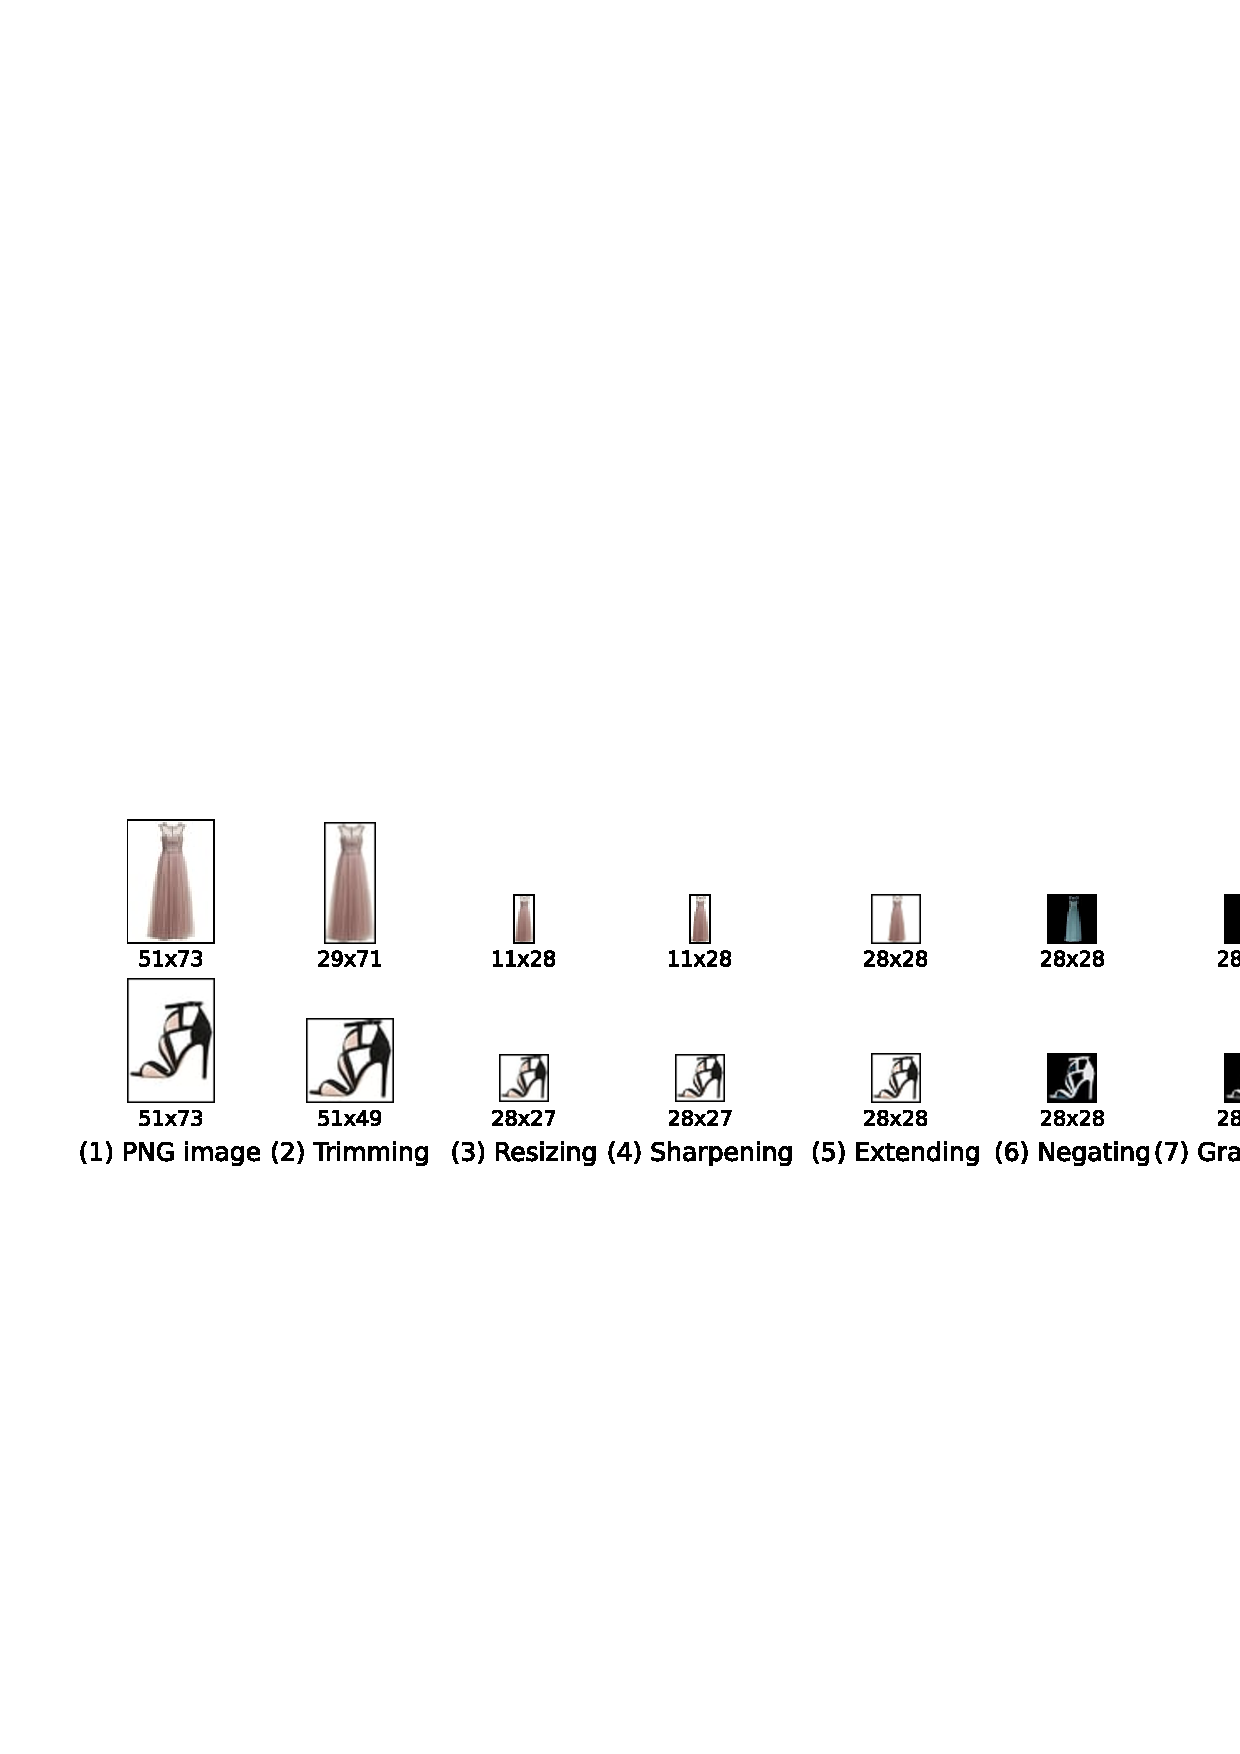
\includegraphics{fig1.png}}
% \caption{Example of a figure caption.}
% \label{fig}
% \end{figure}

% Figure Labels: Use 8 point Times New Roman for Figure labels. Use words 
% rather than symbols or abbreviations when writing Figure axis labels to 
% avoid confusing the reader. As an example, write the quantity 
% ``Magnetization'', or ``Magnetization, M'', not just ``M''. If including 
% units in the label, present them within parentheses. Do not label axes only 
% with units. In the example, write ``Magnetization (A/m)'' or ``Magnetization 
% \{A[m(1)]\}'', not just ``A/m''. Do not label axes with a ratio of 
% quantities and units. For example, write ``Temperature (K)'', not 
% ``Temperature/K''.

% \section*{Acknowledgment}

% The preferred spelling of the word ``acknowledgment'' in America is without 
% an ``e'' after the ``g''. Avoid the stilted expression ``one of us (R. B. 
% G.) thanks $\ldots$''. Instead, try ``R. B. G. thanks$\ldots$''. Put sponsor 
% acknowledgments in the unnumbered footnote on the first page.

% \section*{References}

% Please number citations consecutively within brackets \cite{b1}. The 
% sentence punctuation follows the bracket \cite{b2}. Refer simply to the reference 
% number, as in \cite{b3}---do not use ``Ref. \cite{b3}'' or ``reference \cite{b3}'' except at 
% the beginning of a sentence: ``Reference \cite{b3} was the first $\ldots$''

% Number footnotes separately in superscripts. Place the actual footnote at 
% the bottom of the column in which it was cited. Do not put footnotes in the 
% abstract or reference list. Use letters for table footnotes.

% Unless there are six authors or more give all authors' names; do not use 
% ``et al.''. Papers that have not been published, even if they have been 
% submitted for publication, should be cited as ``unpublished'' \cite{b4}. Papers 
% that have been accepted for publication should be cited as ``in press'' \cite{b5}. 
% Capitalize only the first word in a paper title, except for proper nouns and 
% element symbols.

% For papers published in translation journals, please give the English 
% citation first, followed by the original foreign-language citation \cite{b6}.



\begin{thebibliography}{00}

\bibitem{b1} L. Bregman, “The relaxation method of finding the common point of convex sets and its application to the solution of problems in convex programming,” USSR Computational Mathematics and Mathematical Physics, Volume 7, Issue 3, 1967, pp. 200–217.

\bibitem{b2} J. MacQueen, “Some methods for classification and analysis of multivariate observations," in Proceedings of the Fifth Berkeley Symposium on Mathematical Statistics and Probability, Volume 1 (Univ. of Calif. Press, 1967), pp. 281-297.

\bibitem{b3} R. Xu, D. Wunsch, “Survey of clustering algorithms," IEEE Transactions on Neural Networks, Volume 16, Issue 3, May 2005, pp. 645-678.

\bibitem{b4} J. C. Bezdek, R. Ehrlich, W. Full, “FCM: The fuzzy c-means clustering algorithm," Computers \& Geosciences, Volume 10, Issues 2–3, 1984, pp. 191-203.

\bibitem{b5} D. C. Park, I. Dagher, “Gradient based fuzzy c-means (GBFCM) algorithm," in Proceedings of 1994 IEEE International Conference on Neural Networks (ICNN’94), Volume 3, IEEE, 1994, pp. 1626–1631.

\bibitem{b6} T. Kohonen, “The self-organizing map," in Proceedings of the IEEE, Volume 78, Issue 9, Sept. 1990, pp. 1464-1480.

\bibitem{b7} D. Arthur, S. Vassilvitskii, “K-Means++: the advantages of careful seeding," in Proceedings of The Eighteenth Annual ACM-SIAM Symposium on Discrete Algorithms, Jan. 2007, pp. 1027–1035.

\bibitem{b8} P. Fänti, S. Sieranoja, “K-Means properties on six clustering benchmark datasets," Applied Intelligence, Volume 48, Issue 12, Dec. 2018, pp. 4743-4759.

\bibitem{b9} L.-A. Tran, M.-H. Le, “Robust U-Net-based Road Lane Markings Detection for Autonomous Driving," in Proceedings of the International Conference on System Science and Engineering (ICSSE), July 2019, pp. 62-66.

\end{thebibliography}





% \begin{thebibliography}{00}
% \bibitem{b1} G. Eason, B. Noble, and I. N. Sneddon, ``On certain integrals of Lipschitz-Hankel type involving products of Bessel functions,'' Phil. Trans. Roy. Soc. London, vol. A247, pp. 529--551, April 1955.
% \bibitem{b2} J. Clerk Maxwell, A Treatise on Electricity and Magnetism, 3rd ed., vol. 2. Oxford: Clarendon, 1892, pp.68--73.
% \bibitem{b3} I. S. Jacobs and C. P. Bean, ``Fine particles, thin films and exchange anisotropy,'' in Magnetism, vol. III, G. T. Rado and H. Suhl, Eds. New York: Academic, 1963, pp. 271--350.
% \bibitem{b4} K. Elissa, ``Title of paper if known,'' unpublished.
% \bibitem{b5} R. Nicole, ``Title of paper with only first word capitalized,'' J. Name Stand. Abbrev., in press.
% \bibitem{b6} Y. Yorozu, M. Hirano, K. Oka, and Y. Tagawa, ``Electron spectroscopy studies on magneto-optical media and plastic substrate interface,'' IEEE Transl. J. Magn. Japan, vol. 2, pp. 740--741, August 1987 [Digests 9th Annual Conf. Magnetics Japan, p. 301, 1982].
% \bibitem{b7} M. Young, The Technical Writer's Handbook. Mill Valley, CA: University Science, 1989.
% \end{thebibliography}

% \vspace{12pt}

% \color{red}
% IEEE conference templates contain guidance text for composing and formatting conference papers. Please ensure that all template text is removed from your conference paper prior to submission to the conference. Failure to remove the template text from your paper may result in your paper not being published.

\end{document}

